Das Balancing, wie man schon im Kapitel \ref{TechnischeGrundlagen} erfahren hat, ist eine wichtige Funktion damit der Akku nicht zerstört wird. Das ganze Balancing sollte möglichst einfach aufgebaut sein und mit dem Mikrocontroller ansteuerbar sein. Wie man in Abbildung \ref{fig:Balancing} sieht, wurde dies mit einer P-Kanal Mosfet Schaltung ermöglicht. Der Widerstand am Drain des P-Kanal Mosfet reguliert den Strom mit welchem die einzelnen Zellen ausgeglichen werden. Damit die Schaltung mit einem Mikrocontroller gesteuert werden kann, brauch es einen N-Kanal Mosfet der das Gate des P-Kanal Mosfet auf Ground zieht. Mit dieser einfachen Schaltung ist es möglich die sechs Zellen des Akku zu balancen.

\begin{figure} [H]
	\centering
	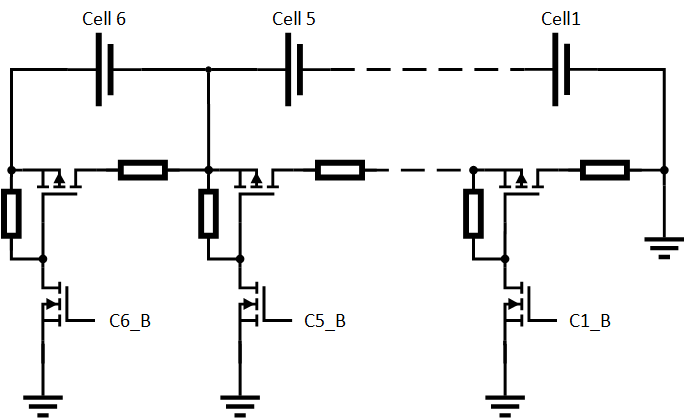
\includegraphics[width=0.6\linewidth]{images/Balancing}
	\caption{Balancing}
	\label{fig:Balancing}
\end{figure}


